\documentclass[authoryear,preprint]{sigplanconf}

\usepackage{amsmath}
\usepackage{tikz}

%vim: set makeprg=runghc make:

%% ODER: format ==         = "\mathrel{==}"
%% ODER: format /=         = "\neq "
%
%
\makeatletter
\@ifundefined{lhs2tex.lhs2tex.sty.read}%
  {\@namedef{lhs2tex.lhs2tex.sty.read}{}%
   \newcommand\SkipToFmtEnd{}%
   \newcommand\EndFmtInput{}%
   \long\def\SkipToFmtEnd#1\EndFmtInput{}%
  }\SkipToFmtEnd

\newcommand\ReadOnlyOnce[1]{\@ifundefined{#1}{\@namedef{#1}{}}\SkipToFmtEnd}
\usepackage{amstext}
\usepackage{amssymb}
\usepackage{stmaryrd}
\DeclareFontFamily{OT1}{cmtex}{}
\DeclareFontShape{OT1}{cmtex}{m}{n}
  {<5><6><7><8>cmtex8
   <9>cmtex9
   <10><10.95><12><14.4><17.28><20.74><24.88>cmtex10}{}
\DeclareFontShape{OT1}{cmtex}{m}{it}
  {<-> ssub * cmtt/m/it}{}
\newcommand{\texfamily}{\fontfamily{cmtex}\selectfont}
\DeclareFontShape{OT1}{cmtt}{bx}{n}
  {<5><6><7><8>cmtt8
   <9>cmbtt9
   <10><10.95><12><14.4><17.28><20.74><24.88>cmbtt10}{}
\DeclareFontShape{OT1}{cmtex}{bx}{n}
  {<-> ssub * cmtt/bx/n}{}
\newcommand{\tex}[1]{\text{\texfamily#1}}	% NEU

\newcommand{\Sp}{\hskip.33334em\relax}


\newcommand{\Conid}[1]{\mathit{#1}}
\newcommand{\Varid}[1]{\mathit{#1}}
\newcommand{\anonymous}{\kern0.06em \vbox{\hrule\@width.5em}}
\newcommand{\plus}{\mathbin{+\!\!\!+}}
\newcommand{\bind}{\mathbin{>\!\!\!>\mkern-6.7mu=}}
\newcommand{\rbind}{\mathbin{=\mkern-6.7mu<\!\!\!<}}% suggested by Neil Mitchell
\newcommand{\sequ}{\mathbin{>\!\!\!>}}
\renewcommand{\leq}{\leqslant}
\renewcommand{\geq}{\geqslant}
\usepackage{polytable}

%mathindent has to be defined
\@ifundefined{mathindent}%
  {\newdimen\mathindent\mathindent\leftmargini}%
  {}%

\def\resethooks{%
  \global\let\SaveRestoreHook\empty
  \global\let\ColumnHook\empty}
\newcommand*{\savecolumns}[1][default]%
  {\g@addto@macro\SaveRestoreHook{\savecolumns[#1]}}
\newcommand*{\restorecolumns}[1][default]%
  {\g@addto@macro\SaveRestoreHook{\restorecolumns[#1]}}
\newcommand*{\aligncolumn}[2]%
  {\g@addto@macro\ColumnHook{\column{#1}{#2}}}

\resethooks

\newcommand{\onelinecommentchars}{\quad-{}- }
\newcommand{\commentbeginchars}{\enskip\{-}
\newcommand{\commentendchars}{-\}\enskip}

\newcommand{\visiblecomments}{%
  \let\onelinecomment=\onelinecommentchars
  \let\commentbegin=\commentbeginchars
  \let\commentend=\commentendchars}

\newcommand{\invisiblecomments}{%
  \let\onelinecomment=\empty
  \let\commentbegin=\empty
  \let\commentend=\empty}

\visiblecomments

\newlength{\blanklineskip}
\setlength{\blanklineskip}{0.66084ex}

\newcommand{\hsindent}[1]{\quad}% default is fixed indentation
\let\hspre\empty
\let\hspost\empty
\newcommand{\NB}{\textbf{NB}}
\newcommand{\Todo}[1]{$\langle$\textbf{To do:}~#1$\rangle$}

\EndFmtInput
\makeatother
%

\begin{document}

%\conferenceinfo{WXYZ '05}{date, City.} 
%\copyrightyear{2005} 
%\copyrightdata{[to be supplied]} 

%\titlebanner{banner above paper title}        % These are ignored unless
%\preprintfooter{short description of paper}   % 'preprint' option specified.

\title{Matrices! Of Types!}
%\subtitle{Subtitle Text, if any}

\authorinfo{Dan Piponi}
           {Google}
           {dpiponi\text{\tt gmail\char46{}com\char125{}~\char92{}authorinfo\char123{}Brent~Yorgey\char125{}~~~~~~~~~~~~\char123{}University~of~Pennsylvania\char125{}~~~~~~~~~~~~\char123{}byorgey}cis.upenn.edu}

\maketitle

\begin{abstract}
Matrices of types are sweet
\end{abstract}

%\category{CR-number}{subcategory}{third-level}

%\terms
%term1, term2

%\keywords
%matrices, types

\section{Introduction}
\label{sec:introduction}

(I'm listing some elementary examples. We don't have to use all of them.)

Here is how we might define a homogeneous list type in Haskell:
\begingroup\par\noindent\advance\leftskip\mathindent\(
\begin{pboxed}\SaveRestoreHook
\column{B}{@{}>{\hspre}l<{\hspost}@{}}%
\column{3}{@{}>{\hspre}l<{\hspost}@{}}%
\column{E}{@{}>{\hspre}l<{\hspost}@{}}%
\>[3]{}\mathbf{data}\;\Conid{List}\;\Varid{a}\mathrel{=}\Conid{Nil}\mid \Conid{Cons}\;\Varid{a}\;(\Conid{List}\;\Varid{a}){}\<[E]%
\ColumnHook
\end{pboxed}
\)\par\noindent\endgroup\resethooks
It's homogeneous because each element has the same type as every other element. But suppose we want some other constraint on our list, for example that the types of the elements alternate between \ensuremath{\Varid{a}} and \ensuremath{\Varid{b}}, starting with \ensuremath{\Varid{a}} and ending with \ensuremath{\Varid{b}}. We can define a pair of mutually recursive types as follows:
\begingroup\par\noindent\advance\leftskip\mathindent\(
\begin{pboxed}\SaveRestoreHook
\column{B}{@{}>{\hspre}l<{\hspost}@{}}%
\column{3}{@{}>{\hspre}l<{\hspost}@{}}%
\column{E}{@{}>{\hspre}l<{\hspost}@{}}%
\>[3]{}\mathbf{data}\;\Conid{AList}\;\Varid{a}\;\Varid{b}\mathrel{=}\Conid{ANil}\mid \Conid{ACons}\;\Varid{a}\;(\Conid{BList}\;\Varid{a}\;\Varid{b}){}\<[E]%
\\
\>[3]{}\mathbf{data}\;\Conid{BList}\;\Varid{a}\;\Varid{b}\mathrel{=}\Conid{BCons}\;\Varid{b}\;(\Conid{AList}\;\Varid{a}\;\Varid{b}){}\<[E]%
\ColumnHook
\end{pboxed}
\)\par\noindent\endgroup\resethooks
The required list is \ensuremath{\Conid{AList}\;\Varid{a}\;\Varid{b}}. Our goal will be to generalise this in two different ways
\begin{itemize}
\item We can think of the sequence of types in our list as conforming to a regular expression $(ab)^\ast$. We can generalize this to other regular expressions.
\item We can consider more general recursive types than lists and make their leaf nodes, when read from left to right, conform to a regular expression
\end{itemize}

\section{An alternating tree}
Let's consider the example of constructing a binary tree whose leaves conform to the regular expression $(ab)^\ast$.

%    ---A->--
%   /        \
% (1)        (2)
%   \        /
%    --<-B---




(Maybe nobody wants to see the gory details of this.)

Here's a basic binary tree:
\begingroup\par\noindent\advance\leftskip\mathindent\(
\begin{pboxed}\SaveRestoreHook
\column{B}{@{}>{\hspre}l<{\hspost}@{}}%
\column{3}{@{}>{\hspre}l<{\hspost}@{}}%
\column{18}{@{}>{\hspre}l<{\hspost}@{}}%
\column{19}{@{}>{\hspre}l<{\hspost}@{}}%
\column{E}{@{}>{\hspre}l<{\hspost}@{}}%
\>[3]{}\mathbf{data}\;\Conid{Tree}\;\Varid{a}\mathrel{=}{}\<[18]%
\>[18]{}\Conid{Leaf}\;\Varid{a}\mid \Conid{Fork}\;(\Conid{Tree}\;\Varid{a})\;(\Conid{Tree}\;\Varid{a}){}\<[E]%
\\
\>[18]{}\hsindent{1}{}\<[19]%
\>[19]{}\mathbf{deriving}\;\Conid{Show}{}\<[E]%
\ColumnHook
\end{pboxed}
\)\par\noindent\endgroup\resethooks
Now suppose that \ensuremath{\Conid{Tree}_{11}} is a tree whose leaf nodes are in $(ab)^\ast$.
(We'll explain the suffix $11$ later.)
It can't itself be a leaf node because then it would have only one element.
It must be a fork consisting of two subtrees.
There are two ways this could happen.
The left fork could start with \ensuremath{\Varid{a}} and end with \ensuremath{\Varid{b}} in which case the right fork must also start with \ensuremath{\Varid{a}} and end with \ensuremath{\Varid{b}}.
Or the left fork could start with \ensuremath{\Varid{a}} and end with \ensuremath{\Varid{a}} in which case the right fork must start with \ensuremath{\Varid{b}} and end with \ensuremath{\Varid{b}}. So we are led to this type:
\begingroup\par\noindent\advance\leftskip\mathindent\(
\begin{pboxed}\SaveRestoreHook
\column{B}{@{}>{\hspre}l<{\hspost}@{}}%
\column{3}{@{}>{\hspre}l<{\hspost}@{}}%
\column{20}{@{}>{\hspre}c<{\hspost}@{}}%
\column{20E}{@{}l@{}}%
\column{23}{@{}>{\hspre}l<{\hspost}@{}}%
\column{31}{@{}>{\hspre}l<{\hspost}@{}}%
\column{45}{@{}>{\hspre}l<{\hspost}@{}}%
\column{E}{@{}>{\hspre}l<{\hspost}@{}}%
\>[3]{}\mathbf{data}\;\Conid{Tree}_{11}\;\Varid{a}\;\Varid{b}{}\<[20]%
\>[20]{}\mathrel{=}{}\<[20E]%
\>[23]{}\Conid{Fork}_{11}\;{}\<[31]%
\>[31]{}(\Conid{Tree}_{11}\;\Varid{a}\;\Varid{b})\;{}\<[45]%
\>[45]{}(\Conid{Tree}_{11}\;\Varid{a}\;\Varid{b}){}\<[E]%
\\
\>[20]{}\mid {}\<[20E]%
\>[23]{}\Conid{Fork}_{11}'\;(\Conid{Tree}_{12}\;\Varid{a}\;\Varid{b})\;{}\<[45]%
\>[45]{}(\Conid{Tree}_{21}\;\Varid{a}\;\Varid{b}){}\<[E]%
\ColumnHook
\end{pboxed}
\)\par\noindent\endgroup\resethooks

Similar reasoning about the subtree types leads to the remainder of the mutually recursive definition:
\begingroup\par\noindent\advance\leftskip\mathindent\(
\begin{pboxed}\SaveRestoreHook
\column{B}{@{}>{\hspre}l<{\hspost}@{}}%
\column{3}{@{}>{\hspre}l<{\hspost}@{}}%
\column{20}{@{}>{\hspre}l<{\hspost}@{}}%
\column{23}{@{}>{\hspre}l<{\hspost}@{}}%
\column{31}{@{}>{\hspre}l<{\hspost}@{}}%
\column{45}{@{}>{\hspre}l<{\hspost}@{}}%
\column{E}{@{}>{\hspre}l<{\hspost}@{}}%
\>[3]{}\mathbf{data}\;\Conid{Tree}_{12}\;\Varid{a}\;\Varid{b}{}\<[20]%
\>[20]{}\mathrel{=}\Conid{Leaf}_{12}\;\Varid{a}{}\<[E]%
\\
\>[20]{}\mid {}\<[23]%
\>[23]{}\Conid{Fork}_{12}\;{}\<[31]%
\>[31]{}(\Conid{Tree}_{11}\;\Varid{a}\;\Varid{b})\;{}\<[45]%
\>[45]{}(\Conid{Tree}_{12}\;\Varid{a}\;\Varid{b}){}\<[E]%
\\
\>[20]{}\mid {}\<[23]%
\>[23]{}\Conid{Fork}_{12}'\;(\Conid{Tree}_{12}\;\Varid{a}\;\Varid{b})\;{}\<[45]%
\>[45]{}(\Conid{Tree}_{22}\;\Varid{a}\;\Varid{b}){}\<[E]%
\ColumnHook
\end{pboxed}
\)\par\noindent\endgroup\resethooks
\begingroup\par\noindent\advance\leftskip\mathindent\(
\begin{pboxed}\SaveRestoreHook
\column{B}{@{}>{\hspre}l<{\hspost}@{}}%
\column{3}{@{}>{\hspre}l<{\hspost}@{}}%
\column{20}{@{}>{\hspre}l<{\hspost}@{}}%
\column{23}{@{}>{\hspre}l<{\hspost}@{}}%
\column{31}{@{}>{\hspre}l<{\hspost}@{}}%
\column{45}{@{}>{\hspre}l<{\hspost}@{}}%
\column{E}{@{}>{\hspre}l<{\hspost}@{}}%
\>[3]{}\mathbf{data}\;\Conid{Tree}_{21}\;\Varid{a}\;\Varid{b}{}\<[20]%
\>[20]{}\mathrel{=}\Conid{Leaf}_{21}\;\Varid{b}{}\<[E]%
\\
\>[20]{}\mid {}\<[23]%
\>[23]{}\Conid{Fork}_{21}\;{}\<[31]%
\>[31]{}(\Conid{Tree}_{21}\;\Varid{a}\;\Varid{b})\;{}\<[45]%
\>[45]{}(\Conid{Tree}_{11}\;\Varid{a}\;\Varid{b}){}\<[E]%
\\
\>[20]{}\mid {}\<[23]%
\>[23]{}\Conid{Fork}_{21}'\;(\Conid{Tree}_{22}\;\Varid{a}\;\Varid{b})\;{}\<[45]%
\>[45]{}(\Conid{Tree}_{21}\;\Varid{a}\;\Varid{b}){}\<[E]%
\ColumnHook
\end{pboxed}
\)\par\noindent\endgroup\resethooks
\begingroup\par\noindent\advance\leftskip\mathindent\(
\begin{pboxed}\SaveRestoreHook
\column{B}{@{}>{\hspre}l<{\hspost}@{}}%
\column{3}{@{}>{\hspre}l<{\hspost}@{}}%
\column{20}{@{}>{\hspre}c<{\hspost}@{}}%
\column{20E}{@{}l@{}}%
\column{23}{@{}>{\hspre}l<{\hspost}@{}}%
\column{31}{@{}>{\hspre}l<{\hspost}@{}}%
\column{45}{@{}>{\hspre}l<{\hspost}@{}}%
\column{E}{@{}>{\hspre}l<{\hspost}@{}}%
\>[3]{}\mathbf{data}\;\Conid{Tree}_{22}\;\Varid{a}\;\Varid{b}{}\<[20]%
\>[20]{}\mathrel{=}{}\<[20E]%
\>[23]{}\Conid{Fork}_{22}\;{}\<[31]%
\>[31]{}(\Conid{Tree}_{21}\;\Varid{a}\;\Varid{b})\;{}\<[45]%
\>[45]{}(\Conid{Tree}_{21}\;\Varid{a}\;\Varid{b}){}\<[E]%
\\
\>[20]{}\mid {}\<[20E]%
\>[23]{}\Conid{Fork}_{22}'\;(\Conid{Tree}_{22}\;\Varid{a}\;\Varid{b})\;{}\<[45]%
\>[45]{}(\Conid{Tree}_{21}\;\Varid{a}\;\Varid{b}){}\<[E]%
\ColumnHook
\end{pboxed}
\)\par\noindent\endgroup\resethooks

Any tree of type \ensuremath{\Conid{Tree}_{11}\;\Varid{a}\;\Varid{b}} is now constrained to have alternating leaf node types:

\begingroup\par\noindent\advance\leftskip\mathindent\(
\begin{pboxed}\SaveRestoreHook
\column{B}{@{}>{\hspre}l<{\hspost}@{}}%
\column{3}{@{}>{\hspre}l<{\hspost}@{}}%
\column{E}{@{}>{\hspre}l<{\hspost}@{}}%
\>[3]{}\Varid{ex}_{1}\mathrel{=}\Conid{Fork}_{11}'\;(\Conid{Leaf}_{12}\;\mathrm{1})\;(\Conid{Leaf}_{21}\;\text{\tt 'a'}){}\<[E]%
\\
\>[3]{}\Varid{ex}_{2}\mathrel{=}\Conid{Fork}_{11}'\;(\Conid{Fork}_{12}\;\Varid{ex}_{1}\;(\Conid{Leaf}_{12}\;\mathrm{2}))\;(\Conid{Leaf}_{21}\;\text{\tt 'b'}){}\<[E]%
\ColumnHook
\end{pboxed}
\)\par\noindent\endgroup\resethooks
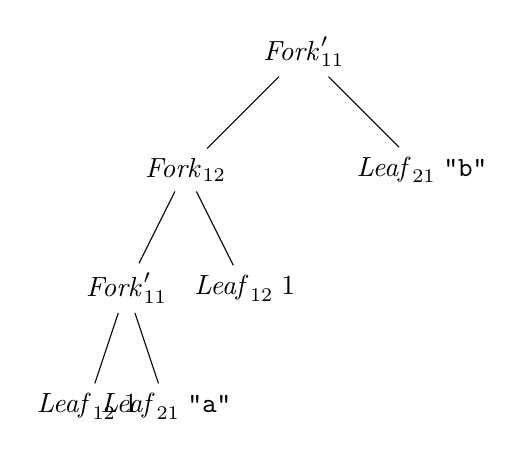
\begin{tikzpicture}[level/.style={sibling distance=30mm/#1}]
\node {\ensuremath{\Conid{Fork}_{11}'}}
  child {
      node {\ensuremath{\Conid{Fork}_{12}}}
          child {node {\ensuremath{\Conid{Fork}_{11}'}}
                    child {node {\ensuremath{\Conid{Leaf}_{12}\;\mathrm{1}}}}
                    child {node {\ensuremath{\Conid{Leaf}_{21}\;\text{\tt \char34 a\char34}}}}
          }
          child {node {\ensuremath{\Conid{Leaf}_{12}\;\mathrm{1}}}}
  }
  child {node {\ensuremath{\Conid{Leaf}_{21}\;\text{\tt \char34 b\char34}}}};
\end{tikzpicture}

While this works, the procedure was somewhat {\it ad hoc}. We reasoned about the properties of the pieces we get when we split a string from $(ab)^\ast$ into two and used this to find corresponding types for the subtrees. Why did we end up with four tree types? And how does this relate to the standard theory of regular languages?

\section{Zippers and dissections}
\label{sec:zippers-and-dissections}

Given a recursive type $t$ we can consider the problem of `lifting' it to a new type that conforms to a given regular expression. It turns out that for certain regular expressions this problem has already been solved in the literature without the problem having been phrased in this form.

Consider the regular language $a^\ast1a^\ast$. It matches sequences of $a$s with precisely one occurrence of $1$ somewhere in the word, where $1$ represents the unit type (usually written \ensuremath{()} in Haskell). Applied to a recursive types it corresponds to trees where all of the leaf nodes are of type \ensuremath{\Varid{a}} apart from one which has the fixed value \ensuremath{()}. In other words, it's the derivative of the orginal type. The regular language $a^\ast ba^\ast$ is a zipper type with elements of type $b$ at the `focus'. And the regular language $a^\ast1b^\ast$ corresponds to dissection types.

Zippers, derivatives and dissections are usually described using Leibniz rules and their generalizations. We'll show how these rules can be placed in a more general framework applying to any regular language.

\section{Matrices of types}
\label{sec:matrices-of-types}

\begin{itemize}
\item Work up to the full solution involving matrices of types.
  Matrices!  Of types!
\end{itemize}

\section{Derivatives, again}
\label{sec:derivatives-again}

\begin{itemize}
\item Circle back round and discuss derivatives, dissection, and
  infinitesimals again from the new vantage point.  (e.g. discuss
  where the usual Leibniz equation comes from.)
\end{itemize}

\section{Divided differences}
\label{sec:divided-differences}

\begin{itemize}
\item Use the new power to also generalize dissections to divided
  differences.
\end{itemize}

\acks

Acknowledgments.

% We recommend abbrvnat bibliography style.

\bibliographystyle{abbrvnat}

\end{document}
